\documentclass[11pt,a4paper]{article}
\usepackage[a4paper,margin=2.4cm]{geometry}
\usepackage[T1]{fontenc}
\usepackage[french]{babel}
\usepackage{lmodern}
\usepackage{graphicx,xcolor,booktabs,array,tabularx}
\usepackage{amsmath}
\usepackage{tikz}
\usetikzlibrary{positioning,arrows.meta,fit,calc}
\usepackage{enumitem,caption,fancyhdr,lastpage,microtype}

\definecolor{accent}{HTML}{8B1E2D}
\definecolor{grisfond}{HTML}{F5F5F7}
\definecolor{grisligne}{HTML}{D6D8DE}
\definecolor{gristexte}{HTML}{5B616B}
\usepackage[colorlinks=true,linkcolor=accent,urlcolor=accent,citecolor=accent]{hyperref}

\captionsetup{font=small,labelfont={bf,color=accent}}
\setlist[itemize]{leftmargin=1.3em,itemsep=2pt,topsep=3pt,parsep=0pt}
\setlist[enumerate]{leftmargin=1.5em,itemsep=2pt,topsep=3pt,parsep=0pt}
\setlength{\parskip}{4pt}
\setlength{\parindent}{0pt}
\emergencystretch=2em
\hbadness=5000

\newcommand{\code}[1]{\texttt{\detokenize{#1}}}

\pagestyle{fancy}\fancyhf{}
\renewcommand{\headrulewidth}{0.4pt}
\fancyhead[L]{\small\textcolor{gristexte}{MedievAIl Battle}}
\fancyhead[R]{\small\textcolor{gristexte}{Rapport technique}}
\fancyfoot[C]{\small\thepage\ / \pageref{LastPage}}

\begin{document}

%================================================================ TITRE
\begin{center}
{\Huge\bfseries\color{accent} MedievAIl Battle}\\[6pt]
{\Large Simulateur de batailles m\'edi\'evales en Python\\[2pt] avec IA, terrains \`a \'el\'evation et analyse de Lanchester}\\[10pt]
{\large Rapport technique}\\[10pt]
{\small Projet collectif STI3A --- INSA Centre-Val de Loire --- octobre 2025 \`a janvier 2026\\
Rapport r\'edig\'e en octobre 2026 \`a partir du d\'ep\^ot, par Mohamed Aziz BAOUEB (\href{https://github.com/aziz3r}{@aziz3r}), mainteneur du miroir\\[2pt]
Code source : \url{https://github.com/aziz3r/medievail-battle}}
\end{center}
\vspace{-2pt}
\noindent\rule{\linewidth}{0.8pt}

\begin{abstract}\noindent
MedievAIl Battle est un jeu de bataille strat\'egique en Python (pygame) o\`u deux arm\'ees d'unit\'es m\'edi\'evales
--- piquiers, chevaliers, arbal\'etriers et, dans un mode particulier, une merveille \`a d\'efendre --- s'affrontent
sur une carte \`a \'el\'evation, pilot\'ees chacune par une intelligence artificielle. Ce document pr\'esente
l'architecture du code, les r\`egles du mod\`ele de combat, les cinq IA livr\'ees, les interfaces (menu, vue isom\'etrique 2.5D,
vue terminal, ligne de commande) et les outils d'analyse (tournois, loi carr\'ee de Lanchester). Il s'appuie
sur des mesures effectu\'ees pour l'occasion --- un tournoi de 500 matchs et des chronom\'etrages --- et signale
les limites rep\'er\'ees dans le code. Le projet est une \oe uvre collective : le d\'ep\^ot est un miroir et
l'historique Git d'origine est conserv\'e.
\end{abstract}

\setcounter{tocdepth}{1}
\tableofcontents

%================================================================ 1
\section{Contexte et objectifs}

MedievAIl Battle a \'et\'e r\'ealis\'e par une \'equipe d'\'etudiants dans le cadre du projet Python / programmation
orient\'ee objet de la formation STI3A \`a l'INSA Centre-Val de Loire. Le d\'ep\^ot de r\'ef\'erence est
\href{https://github.com/awa-b/python-project-2025-2026}{awa-b/python-project-2025-2026} ; celui-ci en est un miroir
maintenu par \href{https://github.com/aziz3r}{@aziz3r} (voir \code{AUTHORS.md} pour la liste des contributeurs
et le d\'etail des droits). L'historique Git compte 111 commits d'\'equipe, du 1\ier{} octobre 2025 au 27 janvier 2026.

Les objectifs, tels qu'ils ressortent du code et de la documentation du d\'ep\^ot, sont les suivants :
\begin{itemize}
  \item mod\'eliser des unit\'es et un combat de fa\c con orient\'ee objet, avec des r\`egles de d\'egats chiffr\'ees
        (bonus de contre, \'el\'evation, pr\'ecision) ;
  \item fournir plusieurs IA interchangeables, pour pouvoir les comparer entre elles ;
  \item offrir plusieurs fa\c cons d'observer une bataille : interface graphique isom\'etrique, terminal, console ;
  \item disposer d'outils d'analyse : tournois automatis\'es et v\'erification des lois de Lanchester.
\end{itemize}

Ce rapport compl\`ete le d\'ep\^ot par une description d'ensemble et une \'evaluation critique. Les chiffres
cit\'es sans r\'ef\'erence ont \'et\'e mesur\'es en octobre 2026 sur un Mac (Python 3.9.6, pygame 2.6.1) ; ils sont
indicatifs, car les batailles comportent une part d'al\'ea (pr\'ecision des arbal\'etriers).

%================================================================ 2
\section{Architecture}

Le code suit un d\'ecoupage \emph{Mod\`ele / Vue / Pr\'esentateur} (MVP). Il repr\'esente environ 5\,800 lignes de Python
(blancs et commentaires inclus) : 1\,769 pour le mod\`ele, 1\,958 pour la vue, 1\,616 pour le pr\'esentateur et 497 pour
les scripts de lancement \`a la racine.

\begin{figure}[h]\centering
\begin{tikzpicture}[font=\scriptsize,>={Stealth},
  boite/.style={draw=grisligne,fill=grisfond,rounded corners=3pt,inner sep=5pt,align=left,text width=4.1cm,minimum height=2.5cm}]
\node[boite] (v) {\textbf{\textcolor{accent}{Vue} --- \texttt{view/}}\\[3pt]
\texttt{menu.py} : menu, lancement\\
\texttt{views.py} : rendu isom\'etrique 2.5D\\
\texttt{terminal\_view.py} : vue curses};
\node[boite,right=8mm of v] (m) {\textbf{\textcolor{accent}{Mod\`ele} --- \texttt{model/}}\\[3pt]
\texttt{game.py} : moteur, \texttt{step}\\
\texttt{map.py} : carte, \'el\'evation\\
\texttt{guerrier.py} et les unit\'es\\
\texttt{terrain.py}, \texttt{scenarios.py},\\
\texttt{army\_compositions.py}};
\node[boite,right=8mm of m] (p) {\textbf{\textcolor{accent}{Pr\'esentateur} --- \texttt{presenter/}}\\[3pt]
\texttt{ai.py}, \texttt{smartAI.py} : 5 IA\\
\texttt{battle.py} : CLI\\
\texttt{tournament.py} : tournois\\
\texttt{graphes\_lanchester.py}};
\draw[->,thick] (v) -- (m);
\draw[->,thick] (p) -- (m);
\draw[->,dashed] (v.north) to[bend left=22] node[above,font=\tiny]{instancie les IA} (p.north);
\end{tikzpicture}
\caption{Organisation du code. La vue lit l'\'etat du mod\`ele et pilote sa boucle ; le pr\'esentateur lit l'\'etat et affecte des ordres aux unit\'es ;
la vue instancie les IA (fl\`eche pointill\'ee). Points d'entr\'ee : \texttt{launch.py}, \texttt{run\_menu.py}, \texttt{visual\_simulation.py}, \texttt{main.py}, \texttt{run\_terminal.py}.}
\end{figure}

\textbf{Un MVP imparfait.} La boucle de simulation (\code{game.step}) est pilot\'ee depuis la vue : c'est
\code{view/menu.py} (fonction \code{start_battle_window}) ou \code{visual_simulation.py} qui l'appelle \`a chaque
image. La vue ne se contente donc pas d'afficher le mod\`ele, elle en cadence l'\'evolution. Ce choix est simple et
efficace pour un jeu, mais il lie le rythme de la simulation \`a celui de l'affichage ; les tournois contournent
le probl\`eme avec leur propre boucle sans affichage.

%================================================================ 3
\section{Le mod\`ele de jeu}

\subsection{Carte et unit\'es}

La carte (\code{BattleMap}, 120$\times$120 par d\'efaut) est \emph{continue} : les unit\'es ont des coordonn\'ees
flottantes \code{(x, y)} et la grille ne sert qu'\`a l'affichage. Seules les bornes sont v\'erifi\'ees lors d'un d\'eplacement :
il n'y a pas de collisions entre unit\'es. L'\'el\'evation est une fonction \code{(x, y)} $\mapsto$ altitude fournie par le terrain.

\begin{table}[h]\centering\small
\begin{tabularx}{\linewidth}{@{}l r X l r r r@{}}
\toprule
Unit\'e & PV & Attaque & Armure & Port\'ee & Vitesse & Recharge \\
\midrule
Chevalier & 100 & 8 (m\^el\'ee) & 2 / 1 & m\^el\'ee & 1,6 & 1,8 s \\
Piquier & 55 & 4 ; +8 contre chevalier & 0 / 0 & m\^el\'ee & 1,1 & 3,0 s \\
Arbal\'etrier & 35 & 5 per\c cante ; +3 contre piquier & 0 / 0 & 7 & 0,96 & 2,0 s \\
Merveille & 4\,800 & --- & 3 / 10 & --- & 0 & --- \\
\bottomrule
\end{tabularx}
\caption{Caract\'eristiques des unit\'es (classes \code{Knight}, \code{Pikeman}, \code{Crossbowman}, \code{Wonder} de \code{model/}). Armure : normale / per\c cante.
Port\'ee : une valeur nulle signifie m\^el\'ee (port\'ee effective d'une tuile). Vision : 4, 4, 9 et 8 tuiles. L'arbal\'etrier a une pr\'ecision de 85\,\% :
un tir manqu\'e consomme tout de m\^eme la recharge. La merveille est immobile et ne riposte pas.}
\end{table}

\subsection{Calcul des d\'egats}

Tous les guerriers h\'eritent de la classe abstraite \code{Guerrier}, qui impl\'emente la formule de d\'egats du sujet :
\[
D \;=\; \max\!\Bigl(1,\; k_{\mathrm{\'elev}}\; \sum_{i} \max\bigl(0,\; A_i - R_i\bigr)\Bigr)
\]
o\`u les $A_i$ sont les composantes d'attaque de l'attaquant (chaque sous-classe en fournit une liste, par exemple
l'attaque de base plus un bonus contre un type de cible) et $R_i$ l'armure correspondante de la cible (normale ou
per\c cante). Le coefficient d'\'el\'evation vaut $k_{\mathrm{\'elev}}=1{,}25$ si l'attaquant est plus haut que sa cible,
$0{,}75$ s'il est plus bas et $1$ sinon. Deux bonus de contre sont cod\'es dans les unit\'es (piquier contre chevalier, arbal\'etrier contre piquier) ; les IA s'appuient sur un cycle de type
pierre-feuille-ciseaux dont elles ajoutent le dernier c\^ot\'e : le chevalier, rapide, rattrape l'arbal\'etrier fragile.

\begin{table}[h]\centering\small
\begin{tabular}{@{}lrrr@{}}
\toprule
Attaquant $\backslash$ cible & Chevalier & Piquier & Arbal\'etrier \\
\midrule
Chevalier & 6 & 8 & 8 \\
Piquier & 8 & 4 & 4 \\
Arbal\'etrier & 4 & 8 & 5 \\
\bottomrule
\end{tabular}
\caption{D\'egats par coup sur terrain plat ($k_{\mathrm{\'elev}}=1$), d\'eduits de la formule et des caract\'eristiques ci-dessus.}
\end{table}

\subsection{Boucle de simulation}

\code{Game.step(dt)} encha\^ine, \`a chaque pas :
\begin{enumerate}
  \item pour chaque \'equipe dont l'intervalle de d\'ecision est \'ecoul\'e, le contr\^oleur d'IA examine l'\'etat et affecte un
        \emph{ordre} (\code{intent}) \`a ses unit\'es : \code{("move_to", x, y)} ou \code{("attack", cible)} ;
  \item les cooldowns des unit\'es vivantes diminuent de \code{dt} ;
  \item chaque unit\'e ex\'ecute son ordre : elle se d\'eplace vers sa destination, ou poursuit sa cible puis frappe si elle est
        \`a port\'ee et si sa recharge est \'ecoul\'ee ;
  \item le temps avance et les conditions de victoire sont test\'ees.
\end{enumerate}
La victoire revient \`a la derni\`ere \'equipe ayant des unit\'es en vie ; dans le mode \emph{Duel de Merveilles}, elle revient \`a
la derni\`ere \'equipe dont la merveille est encore debout. Le moteur cumule aussi des statistiques (d\'egats inflig\'es et subis,
victimes, pertes par type, r\'esum\'e de bataille) et \'ecrit chaque attaque dans un fichier CSV (\code{battle_attacks.txt}).

\subsection{Terrains, compositions et sc\'enarios}

Neuf fonctions de terrain d\'efinissent l'\'el\'evation : plat, colline centrale (\emph{King of the Hill}), deux camps sur
collines sym\'etriques, diagonale, vall\'ee centrale, cr\^ete horizontale, collines al\'eatoires (graine fixe), camp ouest avantag\'e et
si\`ege d'un ch\^ateau central. Cinq compositions d'arm\'ees se combinent avec ces terrains : \emph{Standard} (27 unit\'es par \'equipe),
\emph{Grande Bataille} (105), \emph{Cavalerie lourde} (85), \emph{Archers mass\'es} (100) et \emph{Formation \'equilibr\'ee} (100).
Six sc\'enarios pr\'econfigur\'es sont accessibles depuis le menu (Standard, Grande Bataille, Bataille de la Colline, Deux Camps
\'elev\'es, Si\`ege du Ch\^ateau, Duel de Merveilles), auxquels s'ajoute un sc\'enario $N$ contre $2N$ d\'edi\'e \`a Lanchester.

%================================================================ 4
\section{Les intelligences artificielles}

Cinq contr\^oleurs h\'eritent de \code{BaseController} et diff\`erent par leur crit\`ere de ciblage et par leur fr\'equence de d\'ecision.

\begin{table}[h]\centering\small
\begin{tabularx}{\linewidth}{@{}l r X@{}}
\toprule
IA & D\'ecision & Comportement \\
\midrule
Captain BRAINDEAD & 0,7 s & Ne se d\'eplace jamais ; n'attaque que les ennemis qui viennent \`a port\'ee. \\
Major DAFT & 0,3 s & Charge l'ennemi le plus proche puis l'attaque. \\
Assasin JACK & 0,3 s & Vise l'ennemi le plus faible parmi ceux \`a moins de 15 tuiles, sinon le plus proche. \\
Predict EINSTEIN & 0,15 s & Attribue un score \`a chaque couple unit\'e--ennemi (coups n\'ecessaires pour tuer, bonus de contre, ennemis bless\'es, distance) et concentre les tirs (\emph{focus fire}) sans les sur-concentrer. \\
General STRATEGUS & 0,1 s & R\`egles par type : arbal\'etriers $\to$ piquiers puis arbal\'etriers ; piquiers $\to$ chevaliers ; chevaliers $\to$ arbal\'etriers, avec des seuils de PV pour achever les cibles fragiles. \\
\bottomrule
\end{tabularx}
\caption{Les cinq IA et leur intervalle de d\'ecision (\code{decision_interval}).}
\end{table}

\textbf{Remarque.} Le menu d\'ecrit Predict EINSTEIN comme une IA qui \og simule 5 coups \`a l'avance \fg. Dans le code lu, l'IA
calcule un score instantan\'e pour chaque cible possible et ne simule pas l'\'etat futur du jeu : sa force vient du \emph{focus fire}
et des bonus de contre, non d'une recherche en profondeur. La description du menu gagnerait \`a \^etre mise en conformit\'e.

%================================================================ 5
\section{Interfaces}

\begin{figure}[h]\centering
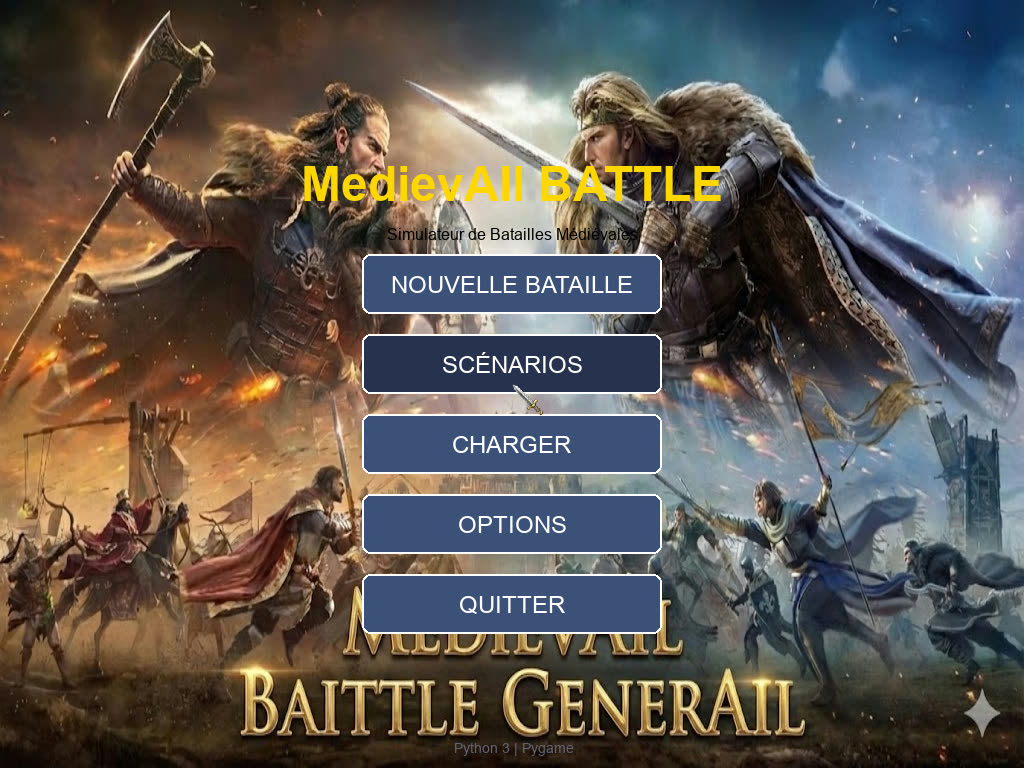
\includegraphics[width=0.48\linewidth]{figures/01_menu_principal.jpg}\hfill
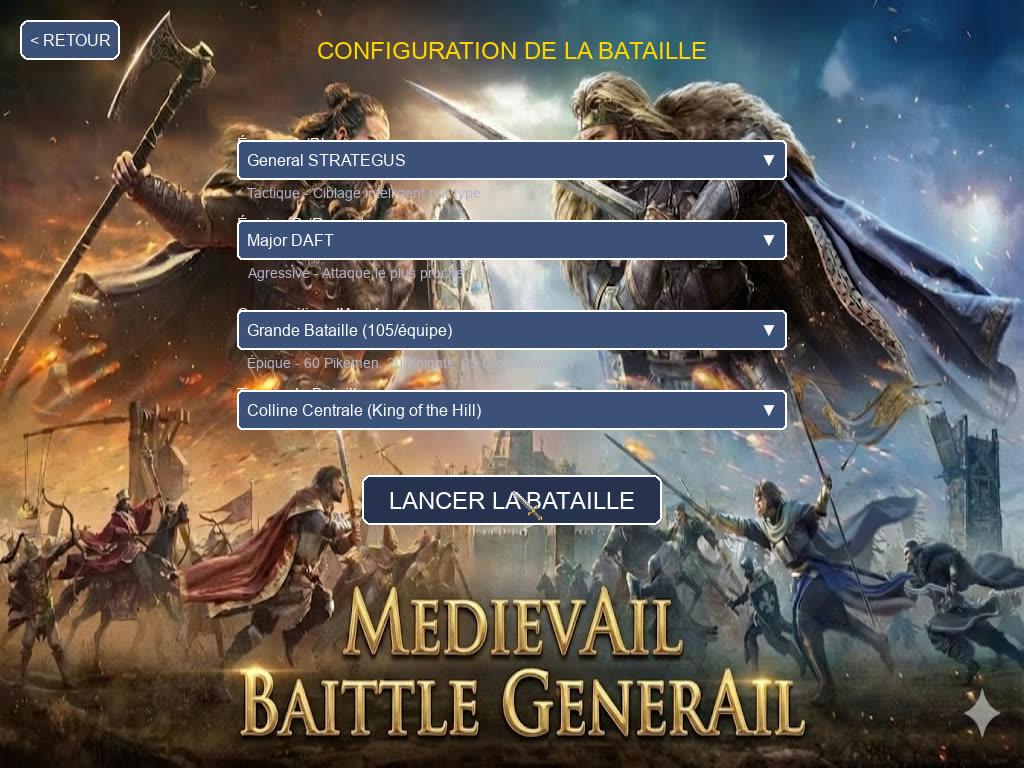
\includegraphics[width=0.48\linewidth]{figures/04_configuration_complete.jpg}\\[4pt]
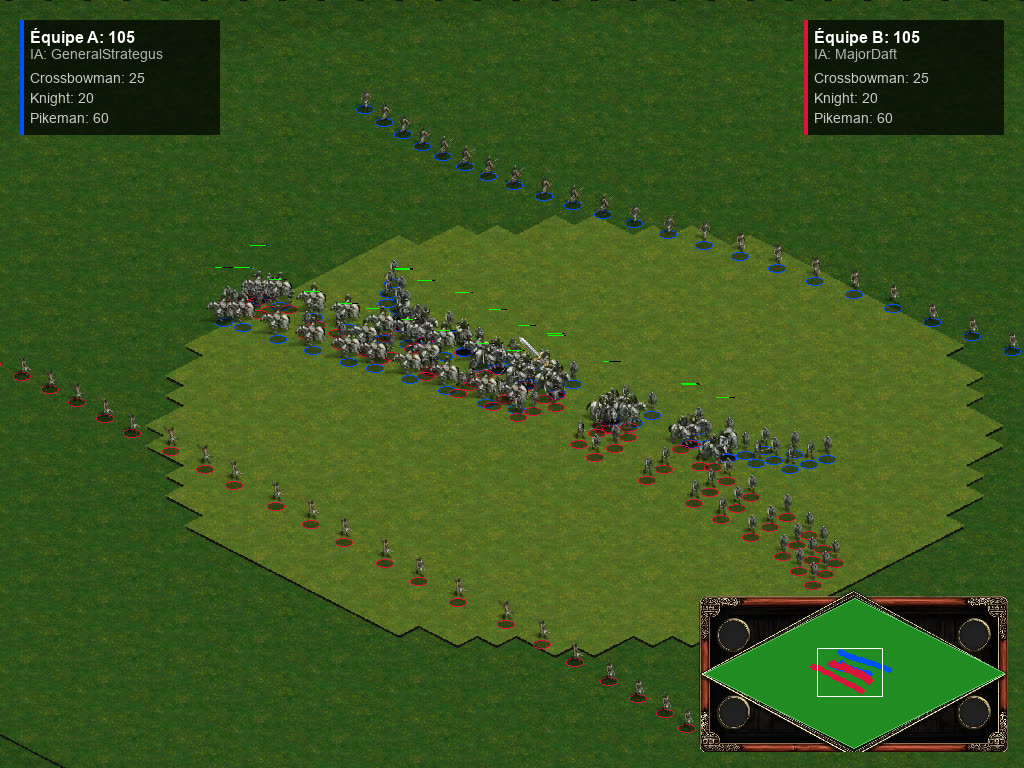
\includegraphics[width=0.48\linewidth]{figures/07_melee.jpg}\hfill
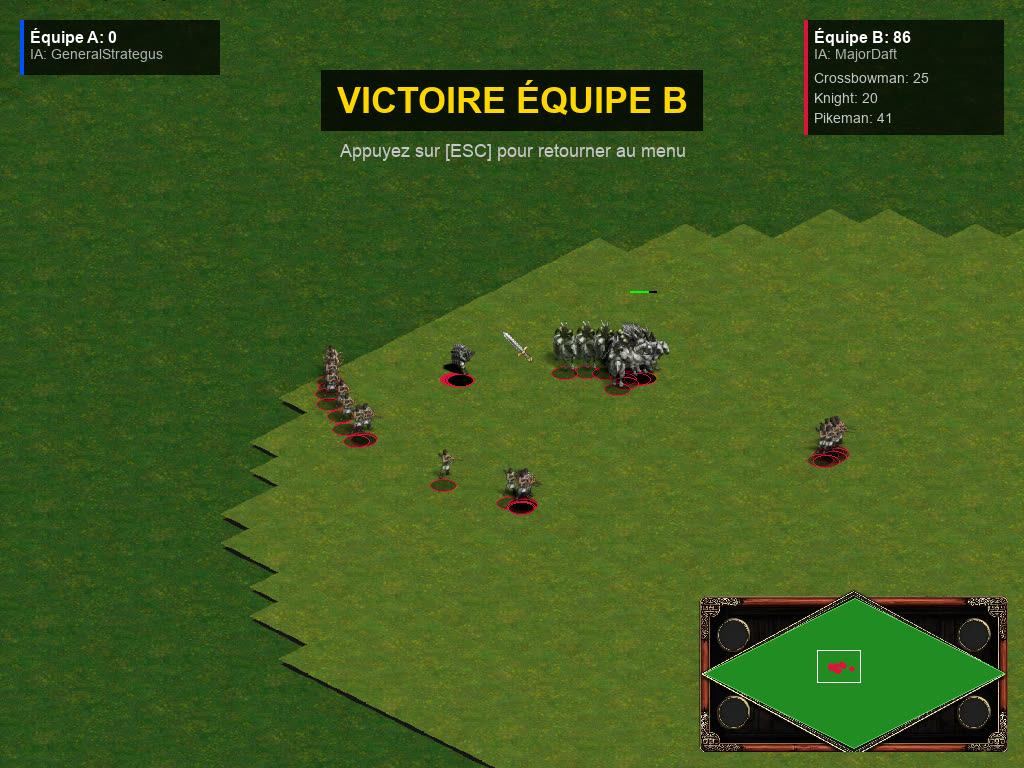
\includegraphics[width=0.48\linewidth]{figures/10_victoire.jpg}
\caption{Parcours du jeu (captures de la d\'emonstration, dossier \code{demo/}) : menu principal, configuration (IA, composition, terrain),
m\^el\'ee entre les deux arm\'ees et \'ecran de victoire.}
\end{figure}

\textbf{Menu pygame} (\code{view/menu.py}). Il propose cinq entr\'ees : nouvelle bataille, sc\'enarios, chargement d'une sauvegarde,
options (vitesse de 10 \`a 120 images par seconde, lecture automatique) et sortie. La configuration d'une bataille permet de choisir
l'IA de chaque camp, la composition et le terrain.

\textbf{Vue isom\'etrique 2.5D} (\code{view/views.py}). Les unit\'es sont dessin\'ees \`a partir de planches de sprites anim\'ees
(repos, marche, attaque, mort, d\'ecomposition) dans seize directions ; le terrain utilise un jeu de tuiles. On peut zoomer \`a la molette
(de 0,1 \`a 2), d\'eplacer la cam\'era \`a la souris ou aux fl\`eches, afficher une minimap (\code{M}), des panneaux de statistiques par arm\'ee
(\code{F1}, \code{F2}, \code{F3}, \code{F4}) et faire une sauvegarde / un chargement rapide (\code{F11}, \code{F12}, format \code{pickle}).

\textbf{Vue terminal} (\code{view/terminal_view.py}), bas\'ee sur \code{curses}, pour observer une bataille sans interface graphique.
\textbf{Ligne de commande} (\code{python -m presenter.battle}) : sous-commandes \code{run}, \code{load}, \code{tourney} et \code{plot}.
Un mode console (\code{main.py}) affiche l'\'etat des arm\'ees dans le terminal.

%================================================================ 6
\section{Exp\'eriences}

\subsection{Tournoi entre les cinq IA}

Le module \code{presenter/tournament.py} joue des matchs sans affichage (pas de 0,2 s, limite de 2\,000 pas, au-del\`a de laquelle le match est nul)
et en alternant les camps \`a chaque manche. Nous l'avons lanc\'e sur le sc\'enario \emph{Standard} (27 unit\'es contre 27), avec 20 manches par confrontation
ordonn\'ee, soit $5\times5\times20 = 500$ matchs, jou\'es en 131 secondes :
\begin{verbatim}
python -m presenter.battle tourney -G Braindead Daft GeneralStrategus \
       AssasinJack PredictEinstein -S Scenario_Standard -N 20
\end{verbatim}

\begin{table}[h]\centering\small\setlength{\tabcolsep}{4pt}
\begin{tabular}{@{}lrrrrrr@{}}
\toprule
Ligne contre colonne (victoires/20) & Brain. & Daft & Strat. & Jack & Eins. & Total/100 \\
\midrule
Predict EINSTEIN & 20 & 20 & 20 & 20 & 11 & \textbf{91} \\
Major DAFT & 20 & 11 & 20 & 17 & 0 & \textbf{68} \\
Assasin JACK & 20 & 3 & 20 & 10 & 0 & \textbf{53} \\
General STRATEGUS & 20 & 0 & 10 & 0 & 0 & \textbf{30} \\
Captain BRAINDEAD & 0 & 0 & 0 & 0 & 0 & \textbf{0} \\
\bottomrule
\end{tabular}
\caption{R\'esultats du tournoi (une ex\'ecution, sc\'enario Standard). Les confrontations miroir (m\^eme IA des deux c\^ot\'es) tournent autour de 50\,\% : 11/20, 10/20, 10/20 et 11/20.}
\end{table}

Le classement est transitif : Einstein $>$ Daft $>$ Jack $>$ Strategus $>$ Braindead. Deux observations m\'eritent d'\^etre not\'ees.
D'abord, Captain BRAINDEAD n'obtient aucune victoire : immobile, il ne peut que subir, et contre lui-m\^eme aucun combat n'a lieu (r\'esultat
coh\'erent avec des matchs nuls). Ensuite, General STRATEGUS, pourtant l'IA la plus \'elabor\'ee \`a r\`egles, perd tous ses matchs contre Daft, Jack et Einstein :
dans ce sc\'enario, une charge simple surpasse un ciblage par type. Nous n'avons pas \'etudi\'e la cause de cet \'ecart ; une hypoth\`ese (non v\'erifi\'ee) est que
la poursuite de cibles sp\'ecifiques disperse les unit\'es. Avec 20 manches par case et un al\'ea sur la pr\'ecision des arbal\'etriers non fix\'e par une graine,
les \'ecarts faibles (par exemple Jack contre Jack) ne sont pas significatifs.

\subsection{Loi carr\'ee de Lanchester}

La loi carr\'ee de Lanchester pr\'edit l'issue d'un combat de masse : si une arm\'ee de $N$ unit\'es identiques affronte une arm\'ee de $2N$, la plus nombreuse
l'emporte et il lui reste $\sqrt{(2N)^2-N^2}=N\sqrt3\approx1{,}73\,N$ survivants. Le module \code{presenter/graphes_lanchester.py} v\'erifie cette pr\'ediction
avec le sc\'enario $N$ contre $2N$ (deux IA Major DAFT, $N$ de 2 \`a 18).

\begin{figure}[h]\centering
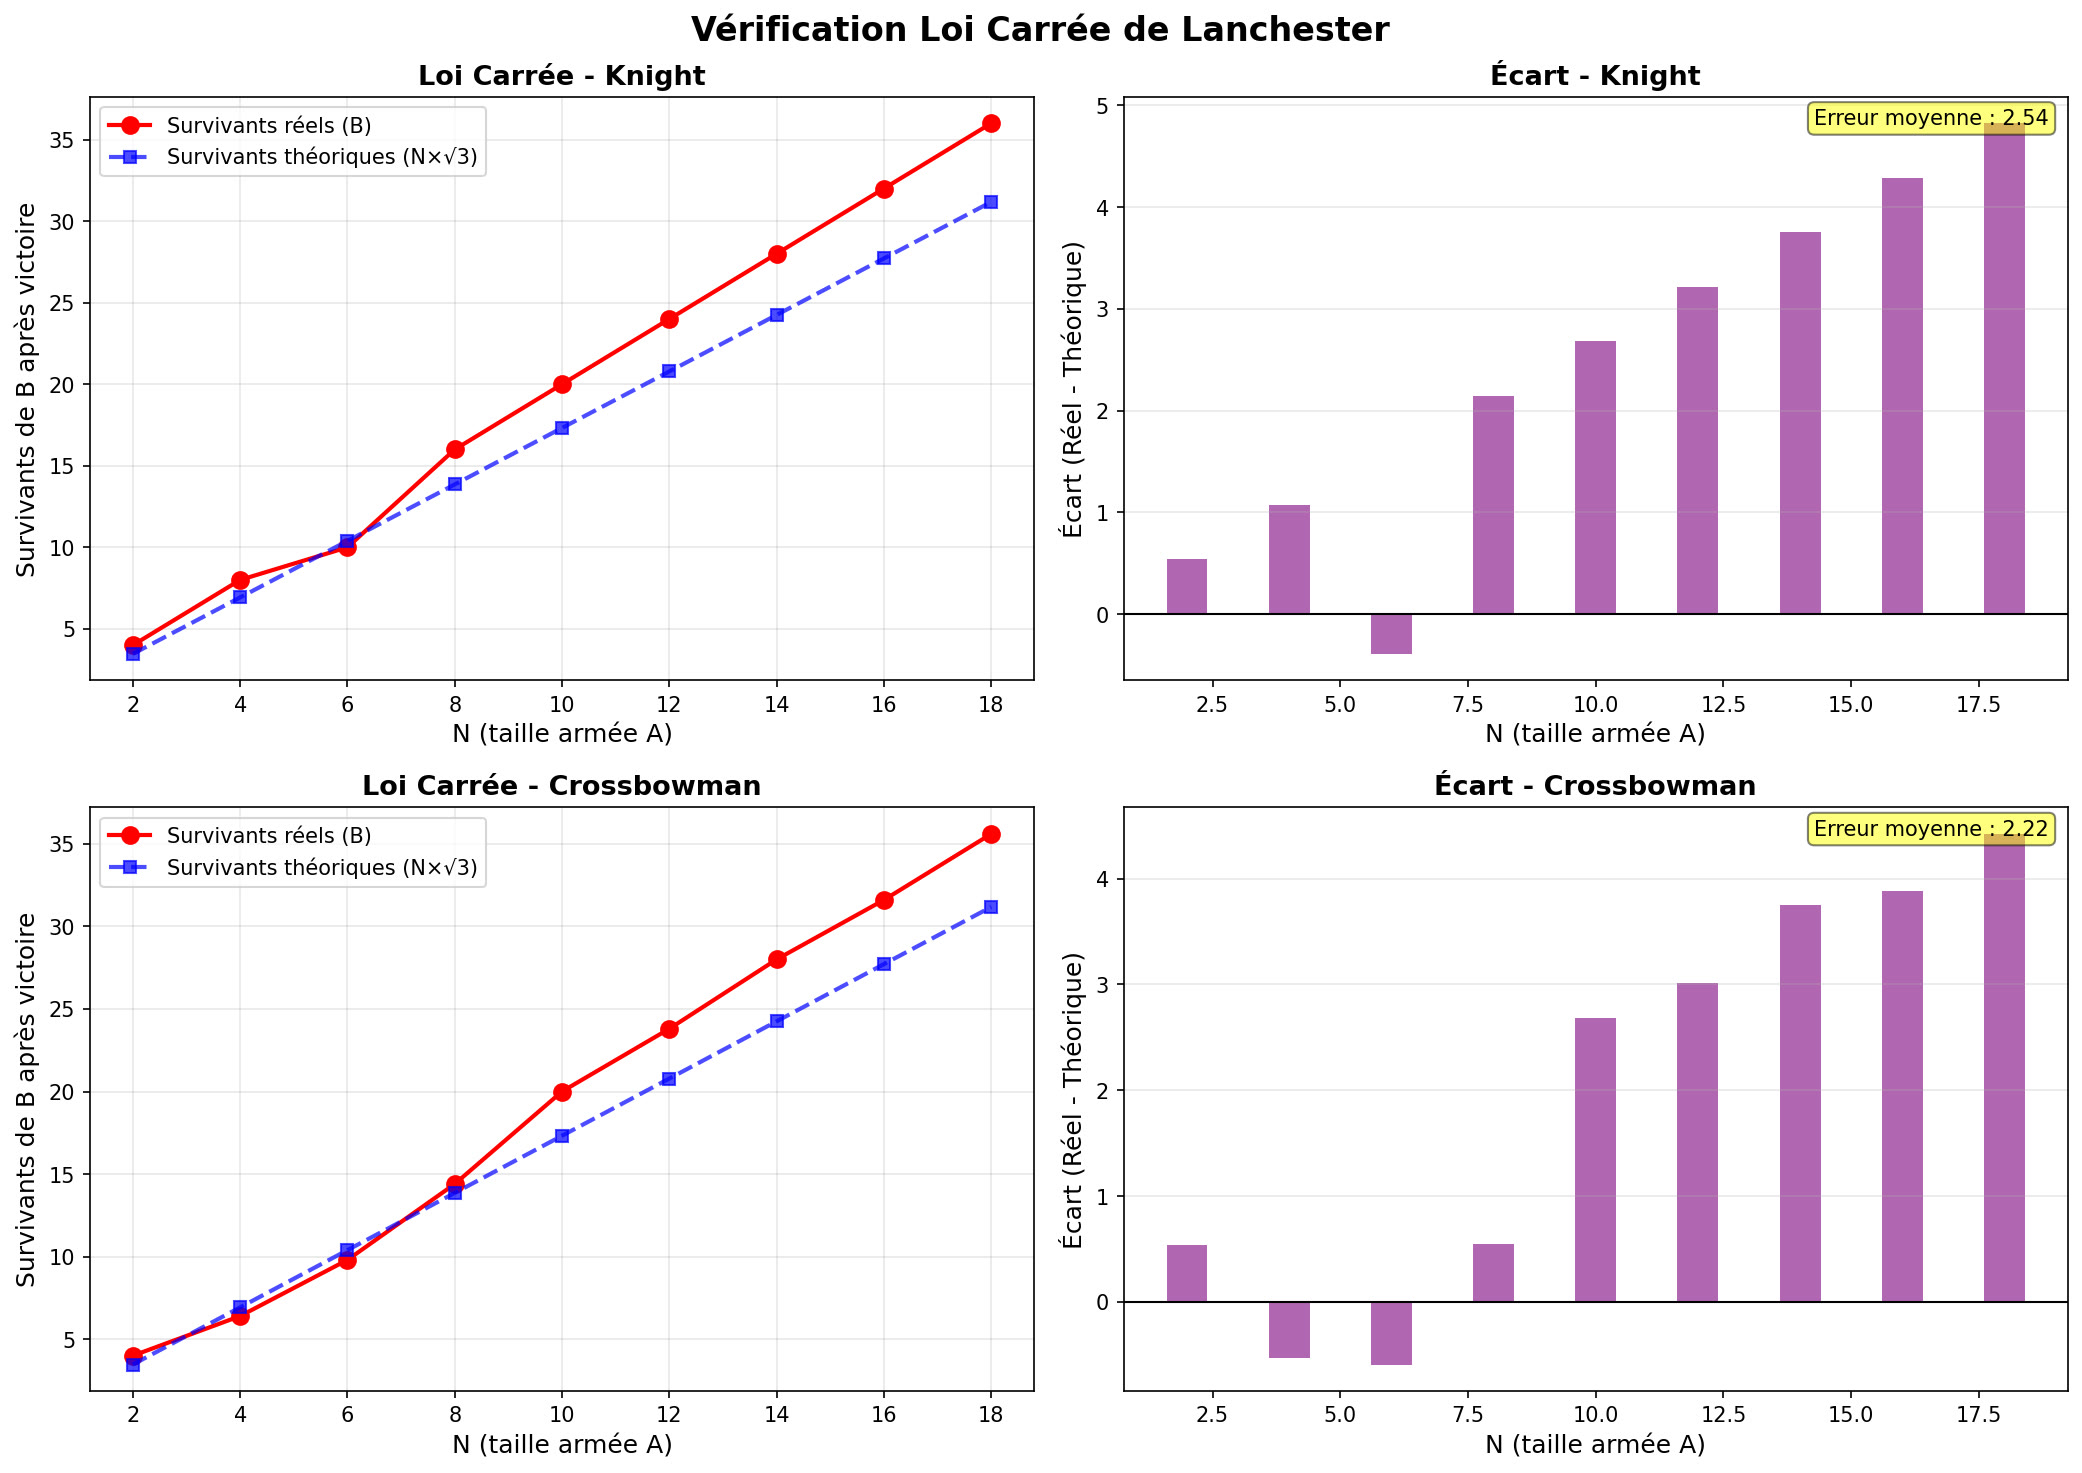
\includegraphics[width=0.95\linewidth]{figures/loi_carree.jpg}
\caption{V\'erification de la loi carr\'ee pour les chevaliers et les arbal\'etriers (fichier \code{loi_carree_knight_crossbowman.png}, d\'ej\`a pr\'esent dans le d\'ep\^ot).
En rouge, survivants r\'eels du camp B ; en bleu, pr\'ediction $N\sqrt3$ ; \`a droite, l'\'ecart.}
\end{figure}

Le r\'esultat ne confirme que partiellement la loi. Le camp le plus nombreux gagne toujours, mais il conserve plus de survivants que pr\'evu : l'\'ecart moyen est de
2,54 survivants pour les chevaliers et de 2,22 pour les arbal\'etriers, et il augmente avec $N$. Sur le graphique, le camp B ne perd presque aucune unit\'e pour les chevaliers.
Nous n'avons pas analys\'e la cause de cet \'ecart ; une piste est que le mod\`ele (d\'eploiement en blocs, absence de collisions, ciblage de l'ennemi le plus proche)
ne produit pas le combat de masse \emph{simultan\'e} dont la loi carr\'ee suppose l'existence.

\subsection{Co\^ut de calcul}

Mesur\'es sans affichage (pas de 0,05 s, terrain \emph{Colline centrale}, General STRATEGUS contre Major DAFT), le sc\'enario Standard (54 unit\'es) se termine en 904 pas
et 0,5 s de calcul ; la Grande Bataille (210 unit\'es) en 1\,056 pas et 6,8 s. Le co\^ut par pas est donc multipli\'e par plus de 10 pour un effectif multipli\'e par 4 :
le ciblage parcourt tous les ennemis pour chaque unit\'e, ce qui est quadratique. Avec l'affichage (rendu sans fen\^etre), la \emph{Grande Bataille} des sc\'enarios classiques tourne \`a environ 22 images par seconde.

%================================================================ 7
\section{D\'emonstration et reproductibilit\'e}

Le dossier \code{demo/} contient une vid\'eo (\code{demo.mp4}, 55 s), un GIF d'aper\c cu, onze captures d'\'ecran et le script \code{capture_demo.py} qui les produit.
Celui-ci ex\'ecute le vrai jeu (menu, configuration puis bataille jusqu'\`a la victoire) avec une entr\'ee pilot\'ee par script et un affichage sans fen\^etre ; la d\'emonstration illustr\'ee ici oppose
General STRATEGUS (A) \`a Major DAFT (B) en Grande Bataille sur la Colline centrale, et se termine par la victoire de l'\'equipe B avec 87 survivants.

Pour lancer le jeu lui-m\^eme (\code{COMMENT_LANCER.md} d\'ecrit toutes les options) :
\begin{verbatim}
pip install pygame
python launch.py              # lanceur interactif
python run_menu_windowed.py   # menu fenetre
python -m presenter.battle run Scenario_Standard Daft Braindead
\end{verbatim}

%================================================================ 8
\section{Limites rep\'er\'ees}

Ces points sont issus de la lecture du code ; ils n'enl\`event rien \`a la r\'eussite d'ensemble du projet.
\begin{itemize}
  \item \textbf{Fichier de journal global.} \code{Game.__init__} \'ecrase \code{battle_attacks.txt} dans le r\'epertoire courant et chaque attaque rouvre le fichier en ajout :
        co\^ut d'entr\'ees-sorties inutile, et impossibilit\'e de jouer deux parties en parall\`ele dans le m\^eme r\'epertoire sans que leurs journaux se m\'elangent.
  \item \textbf{Deux m\'ecanismes d'ordres.} \code{Game.apply_actions} sait ex\'ecuter des actions retourn\'ees par les IA, mais toutes les IA fixent des \code{intent} et renvoient une liste vide :
        ce chemin n'est pas utilis\'e.
  \item \textbf{Option morte du lanceur.} L'entr\'ee 7 de \code{launch.py} lance \code{diagnose_menu.py}, fichier absent du d\'ep\^ot.
  \item \textbf{Aucun test automatis\'e.} Le d\'ep\^ot ne contient pas de tests ; la formule de d\'egats et les conditions de victoire s'y pr\^etent bien.
  \item \textbf{Reproductibilit\'e.} L'al\'ea (pr\'ecision des arbal\'etriers) n'est pas initialis\'e par une graine, donc deux tournois identiques peuvent diff\'erer l\'eg\`erement.
  \item \textbf{Performances.} Ciblage quadratique (parcours de tous les ennemis pour chaque unit\'e), voir la section pr\'ec\'edente.
  \item \textbf{Documentation de l'IA Einstein.} Voir la section~4.
\end{itemize}

%================================================================ 9
\section{Pistes d'am\'elioration}

\begin{enumerate}
  \item Ajouter une graine al\'eatoire param\'etrable et des tests unitaires du moteur (d\'egats, bonus de contre, \'el\'evation, victoire).
  \item Rendre la journalisation optionnelle et tamponn\'ee, ou la confier \`a un objet pass\'e au moteur plut\^ot qu'\`a un fichier global.
  \item R\'eduire le co\^ut du ciblage (grille spatiale ou recherche du plus proche voisin par cases) pour supporter des arm\'ees plus grandes.
  \item Ajouter une gestion minimale des collisions, puis rejouer la v\'erification de Lanchester pour mesurer l'effet sur l'\'ecart \`a la loi carr\'ee.
  \item Si l'on souhaite une IA de recherche, impl\'ementer r\'eellement une simulation de quelques coups ; sinon, corriger la description du menu.
  \item Extraire la boucle de simulation de la vue pour se rapprocher d'un MVP strict.
\end{enumerate}

\end{document}
